\documentclass[11pt]{beamer}
\usepackage[utf8]{inputenc}
\usepackage[T1]{fontenc}
\usepackage{lmodern}
\usepackage[english]{babel}
\usepackage{amsmath}
\usepackage{amsfonts}
\usepackage{amssymb}
\usepackage{graphicx}
\usepackage{hyperref}
\usepackage{color}

\usecolortheme{solarized}
%\usecolortheme[dark]{solarized}

\graphicspath{{img/}}

\begin{document}
	\setbeamertemplate{caption}{\raggedright\insertcaption\par}	% Get rid of "Figure:" label in figures
	\author{ASULUG}
	\title{Introduction to the Command Line Interface}
	\subtitle{A Tutorial On Using the Bash Shell}
	\logo{
\includegraphics[width=.2\textwidth]{asulug-logo.png}}
	\institute{Arizona State University}
	%\date{}
	%\subject{}
	%\setbeamercovered{transparent}
	%\setbeamertemplate{navigation symbols}{}
	\begin{frame}[plain]
	\maketitle
	\begin{figure}
		
\includegraphics[scale=2]{asulug-logo.png}
	\end{figure}
	Made with \LaTeX
\end{frame}

\begin{frame}[t]{What Is A Shell?}
	\begin{columns}
		\begin{column}{0.5\textwidth}
			\begin{itemize}
				\item In computing, a shell is \textit{a user interface} for access to an operating system's services.
				\item Shells can be \textit{graphical} or \textit{text-based}.
				\item It is called a shell because it is the program on the outermost layer around the operating system kernel.
				\begin{itemize}
					\item Applications are started using a command invoked through the shell.
				\end{itemize}
			\end{itemize}
		\end{column}
		\begin{column}{0.5\textwidth}
			\vspace{-5mm}
			\begin{figure}
				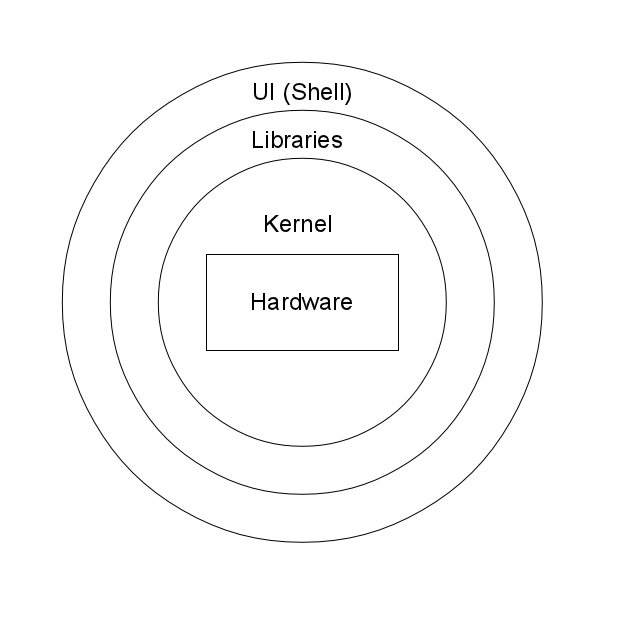
\includegraphics[scale=0.25]{os-layers.png}
				\caption{A simplified, 3-layer layout of a common operating system}
			\end{figure}
		\end{column}
	\end{columns}
\end{frame}

\begin{frame}{Shells vs. Terminals}
	\begin{columns}
		\begin{column}{0.6\textwidth}
			\begin{itemize}
				\item Mid-60's and 70's: one \textit{mainframe computer} shared by many users.
				\item Access the mainframe by one of many \textit{teletype terminals} (\textit{TTY}s), physical devices with a keyboard and screen hard-wired to the mainframe.
				\item TTYs would run a text-based shell to send commands to the mainframe.
				\item Nowadays, a \textit{terminal emulator} (\texttt{gnome-terminal}, \texttt{xterm}, etc.) emulates a physical terminal, which runs a shell.
			\end{itemize}
		\end{column}
		\begin{column}{0.4\textwidth}
			\vspace{-10mm}
			\begin{figure}
				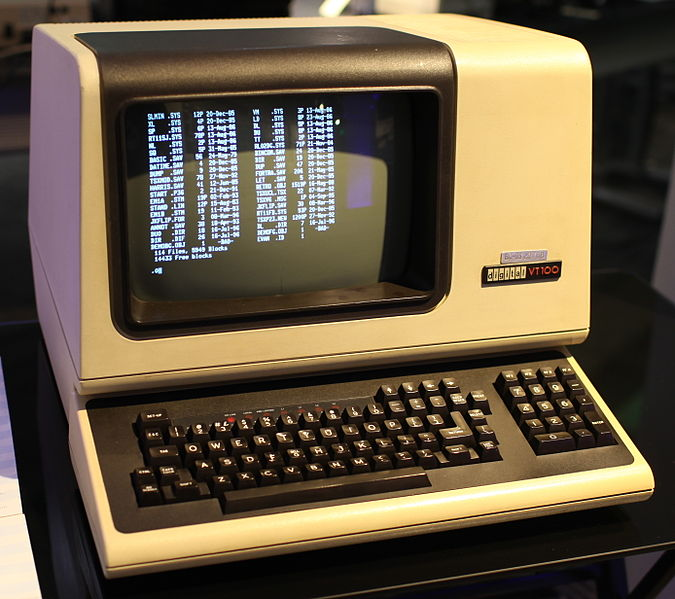
\includegraphics[scale=0.2]{vt100.png}
				\caption{An original VT100 teletype terminal}
			\end{figure}
		\end{column}
	\end{columns}
\end{frame}

\begin{frame}{UNIX-Based Shells}
	\begin{itemize}
		\item \textbf{Thompson Shell} (\texttt{sh}) | The first UNIX shell created by Ken Thompson
		\begin{itemize}
			\item Introduced many basic features such as piping, simple control stuctures (\texttt{if}, \texttt{goto}, etc.), and filename wildcarding (\texttt{*}).
			\item Traditionally located at \texttt{/bin/sh} on older UNIX systems.
		\end{itemize}
		\item \textbf{Bourne Shell} (\texttt{sh}) | A rewrite of the Thompson shell with more features common to modern shells today.
		\begin{itemize}
			\item Introduced more features such as here documents, command substitution, more generic variables and more extensive builtin control structures.
		\end{itemize}
		\color{blue} \item \textbf{Bourne-Again Shell} (\texttt{bash}) | The GNU project's replacement of the Bourne Shell.
	\end{itemize}
\end{frame}
\end{document}